%---------------------------------
%---------------------------------
\chapter{Biologie der Wirbeltiere}
\label{chapter:biology}
% eventuell als Abschnitt in "`Grundlagen"'?

\begin{center}
 \begin{minipage}{12cm}
  \emph{"`Nichts anderes in der Natur hat eine herrlichere Struktur als der Körper der Wirbeltiere."'}
 
  --- "`Vergleichende und funktionelle Anatomie der Wirbeltiere"' \cite{Vergleichende_Anatomie}, S.\ 1
 \end{minipage}
\end{center}

Dieses Kapitel soll einen Überblick über die biologische Beschaffenheit der Wirbeltiere geben. Da dies keine biologische Arbeit ist, werden nur diejenigen Merkmale und Eigenschaften weiter ausgeführt, die im Folgenden zum Verständnis nötig sind.

% Definition
Wirbeltiere, oder auch Vertebrata, sind Tiere mit einer skelettartigen Schädelkapsel, einem Cranium. Deshalb werden sie auch Schädeltiere oder Craniota genannt.\\
Auf den ersten Blick ist diese Definition etwas überraschend, da als  Haupteigenschaft nicht die Wirbelsäule, sondern der Schädel genannt wird. Das liegt daran, dass zu den Wirbeltieren auch einige Tiere gezählt werden, die gar keine Wirbelsäule sondern "`nur"' eine Chorda dorsalis besitzen. Die Chorda dorsalis ist das Achsenskelett der Chordatiere, einem Tierstamm, zu dem auch die Wirbeltiere gehören. (\cite{Vergleichende_Anatomie}, S.27)\\ %und Wikipedia zu Wirbeltieren und chorda dorsalis
Hier in dieser Arbeit soll es aber nur um Wirbeltiere mit Wirbelsäule gehen.

% 5 Klassen
Es gibt fünf große Gruppen von Wirbeltieren. Die ersten bekannten Wirbeltiere sind die Fische. Aus ihnen entwickelten sich die Tetrapoden, Wirbeltiere mit vier Gliedmaßen, zu denen alle anderen Gruppen gehören. Zunächst entstanden die Amphibien, die noch nicht vollkommen terrestrisch leben. Daraus entwickelten sich die Reptilien, die erste Klasse der Wirbeltiere, die alle Strukturen besitzt um vollkommen an Land zu leben. (Es gibt aber auch Reptilien die trotzdem wieder im Wasser leben.) Außerdem gibt es noch die Klassen der Vögel und der Säugetiere.

Das weithin bekannteste Säugetier ist der Mensch. Da sich Wirbeltiere, vor allem in ihrem Skelett, sehr ähneln, lassen sich viele der im Folgenden aufgeführten Eigenschaften vermutlich leicht "`am eigenen Leib"' nachvollziehen.


%------------------------------------
\section{Das Skelett}
\label{biology_skeleton}

\vspace{0.5cm}
\begin{center}
 \begin{minipage}{12cm}
  \emph{"`Das innere, gelenkige Skelettsystem der Vertebraten ist einzigartig im Tierreich. Es ist das wichtigste aller Organsysteme für das Studium der Wirbeltiermorphologie."'}
  --- \cite{Vergleichende_Anatomie}, S.\ 131
 \end{minipage}
\end{center}

Wirbeltiere haben ein inneres Skelett und ihr Körper ist bilateralsymmetrisch. Das bedeutet, dass ihre linke Körperseite symmetrisch zur rechten ist. 

% Wirbelsäule
Die \emph{Wirbelsäule} ist je nach Lebensweise des entsprechenden Wirbeltiers aufgebaut. Ein wesentlicher Einflussfaktor auf Form und Aufbau sind die Kräfte, die auf sie wirken. 
Bei Fischen muss die Wirbelsäule dem Druck der starken Axialmuskeln, die seitlich am Körper entlang führen, entgegenwirken.
Bei Tetrapoden sind diese Axialmuskeln zurückgebildet, dafür muss die Wirbelsäule aber der Schwerkraft widerstehen.
Bei Vögeln ist die Wirbelsäule noch einmal mehr spezialisiert, da sie an den Flug angepasst werden muss.

% Wirbelanzahl
Auch die Anzahl der Wirbel unterscheidet sich teilweise erheblich. 
Die Halswirbelsäule ist \zb bei den Fischen noch gar nicht herausgebildet. Amphibien haben einen Wirbel, der für die Beweglichkeit des Kopfes zuständig ist. Bei Reptilien ist die Halsregion meist schon stärker abgesetzt. Säugetiere haben, bis auf wenige Ausnahmen, genau $7$ Halswirbel, egal wie lang der Hals ist. Vögel haben die meisten Halswirbel, nämlich $10$ bis maximal $31$ beim Trauerschwan \cite{WikipediaVogelskelett}, meistens aber zwischen $15$ und $20$. (siehe auch \cite{Vergleichende_Anatomie}, Abschnitt 9.2, S.\ 168 ff.)

Ebenso unterscheidet sich die Anzahl der Wirbel auf anderen Teilen der Wirbelsäule. Teilweise sind Wirbel sogar miteinander zu einem größeren Knochen verwachsen. Betrachtet man nur die Gruppe der Säugetiere, so kommt man auf auf etwa $12$ bis $14$ Brustwirbel, $5$ bis $7$ Lendenwirbel, $3$ bis $5$ Kreuzwirbel und $4$ bis $22$ Schwanzwirbel \cite{AnatomieKuenstler}.

% Wirbelform
Auch die Form der einzelnen Wirbel unterscheidet sich sowohl zwischen den verschiedenen Tieren als auch entlang der Wirbelsäule einer einzelnen Art (\cite{Vergleichende_Anatomie}, Abschnitt 9.1 und Abbildung 9.2). Diese Vielfalt in ein Regelwerk zu zwängen, um sie automatisch generieren zu können, erscheint aussichtslos. Deshalb wird hier nicht weiter darauf eingegangen.

% Extremitäten
Die \emph{Extremitäten} der Tetrapoden sind nach einem "`Grundbauplan"' aufgebaut (siehe Abbildung \ref{grundbauplan}). Dieser wird jedoch vielfach abgewandelt. Einige Beispiele sind in Abbildung \ref{bsp_extremitaeten} zu sehen. (\cite{AllgemeineZoologie}, S.\ 487)\\
Bei Fischen haben die Extremitäten keine Verbindung zur Wirbelsäule. Erst Amphibien bilden hier eine Verbindung, da sie zur Fortbewegung an Land nötig ist. Dies wird im Folgenden, der Einfachheit halber, aber nicht weiter beachtet. (\cite{Vergleichende_Anatomie}, Abschnitt 9.2.3)

\begin{figure}
 \centering
 \includegraphics[width=0.8\textwidth]{graphics/GrundbauplanExtremitaet.pdf}
 \caption{\emph{Grundbauplan} der Extremitäten von Tetrapoden: Humerus = Oberarmknochen, Femur = Oberschenkelknochen, Radius = Speiche, Ulna = Elle, Tibia = Schienbein, Fibula = Wadenbein, Metacarpus = Mittelhand, Metatarsus = Mittelfuß. (\cite{AllgemeineZoologie}, S.\ 487; eine ähnliche Abbildung ist auch in \cite{Vergleichende_Anatomie}, S.\ 184, zu finden)}
 \label{grundbauplan}
\end{figure}

\begin{figure}
 \centering
 \includegraphics[width=0.8\textwidth]{graphics/ExtremitaetenBeispiele2.pdf}
 \caption{Vordergliedmaßen von Mensch (1), Eidechse (2), Wal (3), Maulwurf (4), Pinguin (5), Pferd (6), Flugsaurier (7), Vogel (8) und Fledermaus (9). (\cite{dtvBiologie}, S.\ 474)}
 \label{bsp_extremitaeten}
\end{figure}

% Extremitätengürtel
Schulter- und Beckengürtel bestehen  jeweils aus mehreren Knochen, die je nach Art mehr oder weniger ausgebildet, unterschiedlich geformt oder sogar komplett zurückgebildet sein können (siehe \cite{Vergleichende_Anatomie}, Absatz 9.7). Um das im Folgenden zu vereinfachen, wird der Schultergürtel durch ein Schulterblatt repräsentiert und der Beckengürtel durch einen "`Beckenknochen"', der allerdings eigentlich auch wieder aus mehreren Einzelknochen besteht.

% verallgemeinerter und abstrahierter Bauplan
Das Skelett von Wirbeltieren ist im Allgemeinen also ein kompliziertes Konstrukt aus vielen Einzelteilen, die auch zwischen verschiedenen Arten stark variieren. Um einen Algorithmus zu entwerfen, der solche Gebilde konstruiert, ist es also notwendig ein erheblich einfacheres Modell zu erstellen.\\ 
In Abbildung \ref{bauplan_skelett} ist ein ein verallgemeinerter und abstrahierter Bauplan für Wirbeltiere zu sehen. Er ist reduziert auf die Wirbelsäule, Rippen, Schädel, Extremitäten, Hüft- und Schultergürtel. Die Extremitäten bestehen jeweils aus Oberarm/-schenkel, Unterarm/Schienbein und Hand/Fuß. Hände und Füße werden hier jeweils als ein "`Knochen"' betrachtet, obwohl sie natürlich aus vielen Einzelteilen bestehen. Es kann maximal zwei Extremitätenpaare geben, jeweils einer an jedem Extremitätengürtel. Rippen, Hals- und Schwanzwirbelsäule sind optional und auch die Anzahl der Wirbel und Rippen variiert je nach Tier.

\begin{figure}
 \centering
 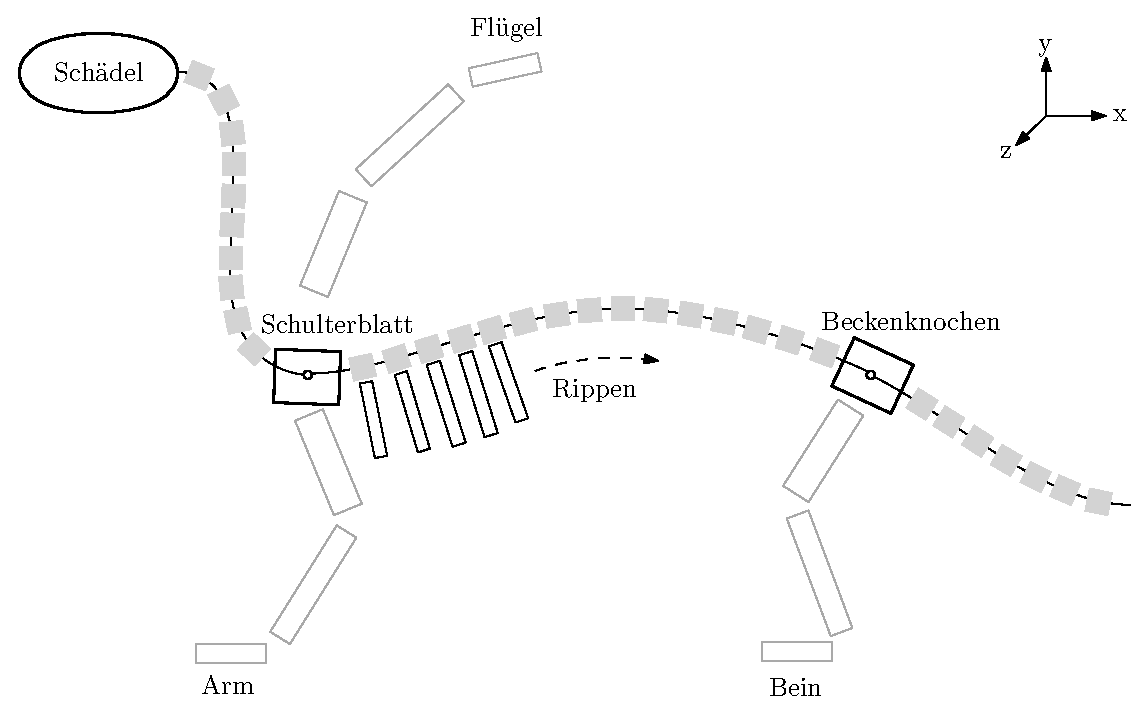
\includegraphics[width=\textwidth]{graphics/skeletonPlan}
 \caption{Verallgemeinerter und abstrahierter Bauplan eines Wirbeltierskeletts. Es sind zwei Extremitätenpaare erlaubt, jeweils einer an jedem Extremitätengürtel. Rippen und Hals- und Schwanzwirbelsäule sind optional. Die Anzahl der Wirbel und Rippen variiert je nach Tier.}
 \label{bauplan_skelett}
\end{figure}


%Gelenke
Auch bei \emph{Gelenken} gibt es viele verschiedene Ausprägungen (siehe \cite{Vergleichende_Anatomie}, Absatz 21.5.2). Der Einfachheit halber werden hier nur drei Arten von Gelenken betrachtet: unbewegliche Gelenke (\zb zwischen Wirbeln), Gelenke mit einem Freiheitsgrad (\zb an Ellenbogen oder Knie) und Gelenke mit zwei Freiheitsgraden (\zb an Schulter oder Hüfte).
Im vereinfachten Modell sind alle Gelenke unbeweglich, bis auf diejenigen in Extremitäten. Außerdem wird angenommen, dass die jeweiligen Bewegungsradien für alle Wirbeltiere gleich sind. 

Im Folgenden sind vor allem die möglichen Winkel der Gelenke in einer Ruheposition des Skeletts von Interesse. Diese sind in Abbildung \ref{joints} visualisiert. Schulter- und Hüftgelenk können eigentlich auch von der Körperachse wegbewegt werden. Diese Bewegungsrichtung wurde dann aber nicht verwendet. Deshalb ist sie hier nicht dargestellt.

\begin{figure}
  \subfloat{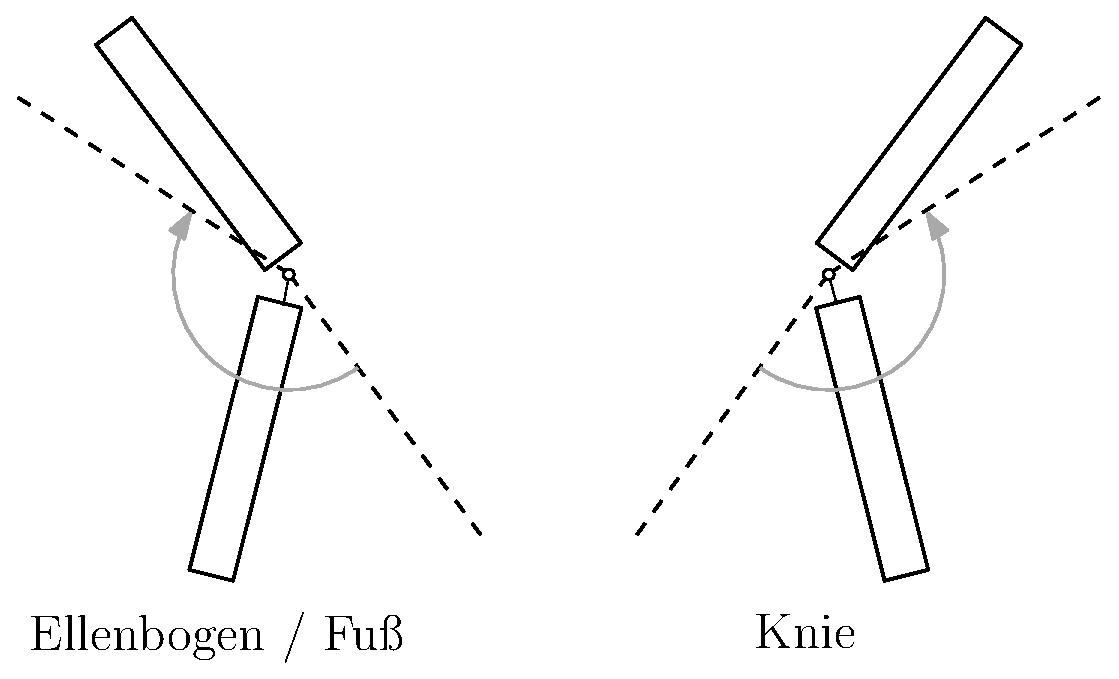
\includegraphics[width=0.5\textwidth]{graphics/oneDimJoints}}
  \qquad
  \subfloat{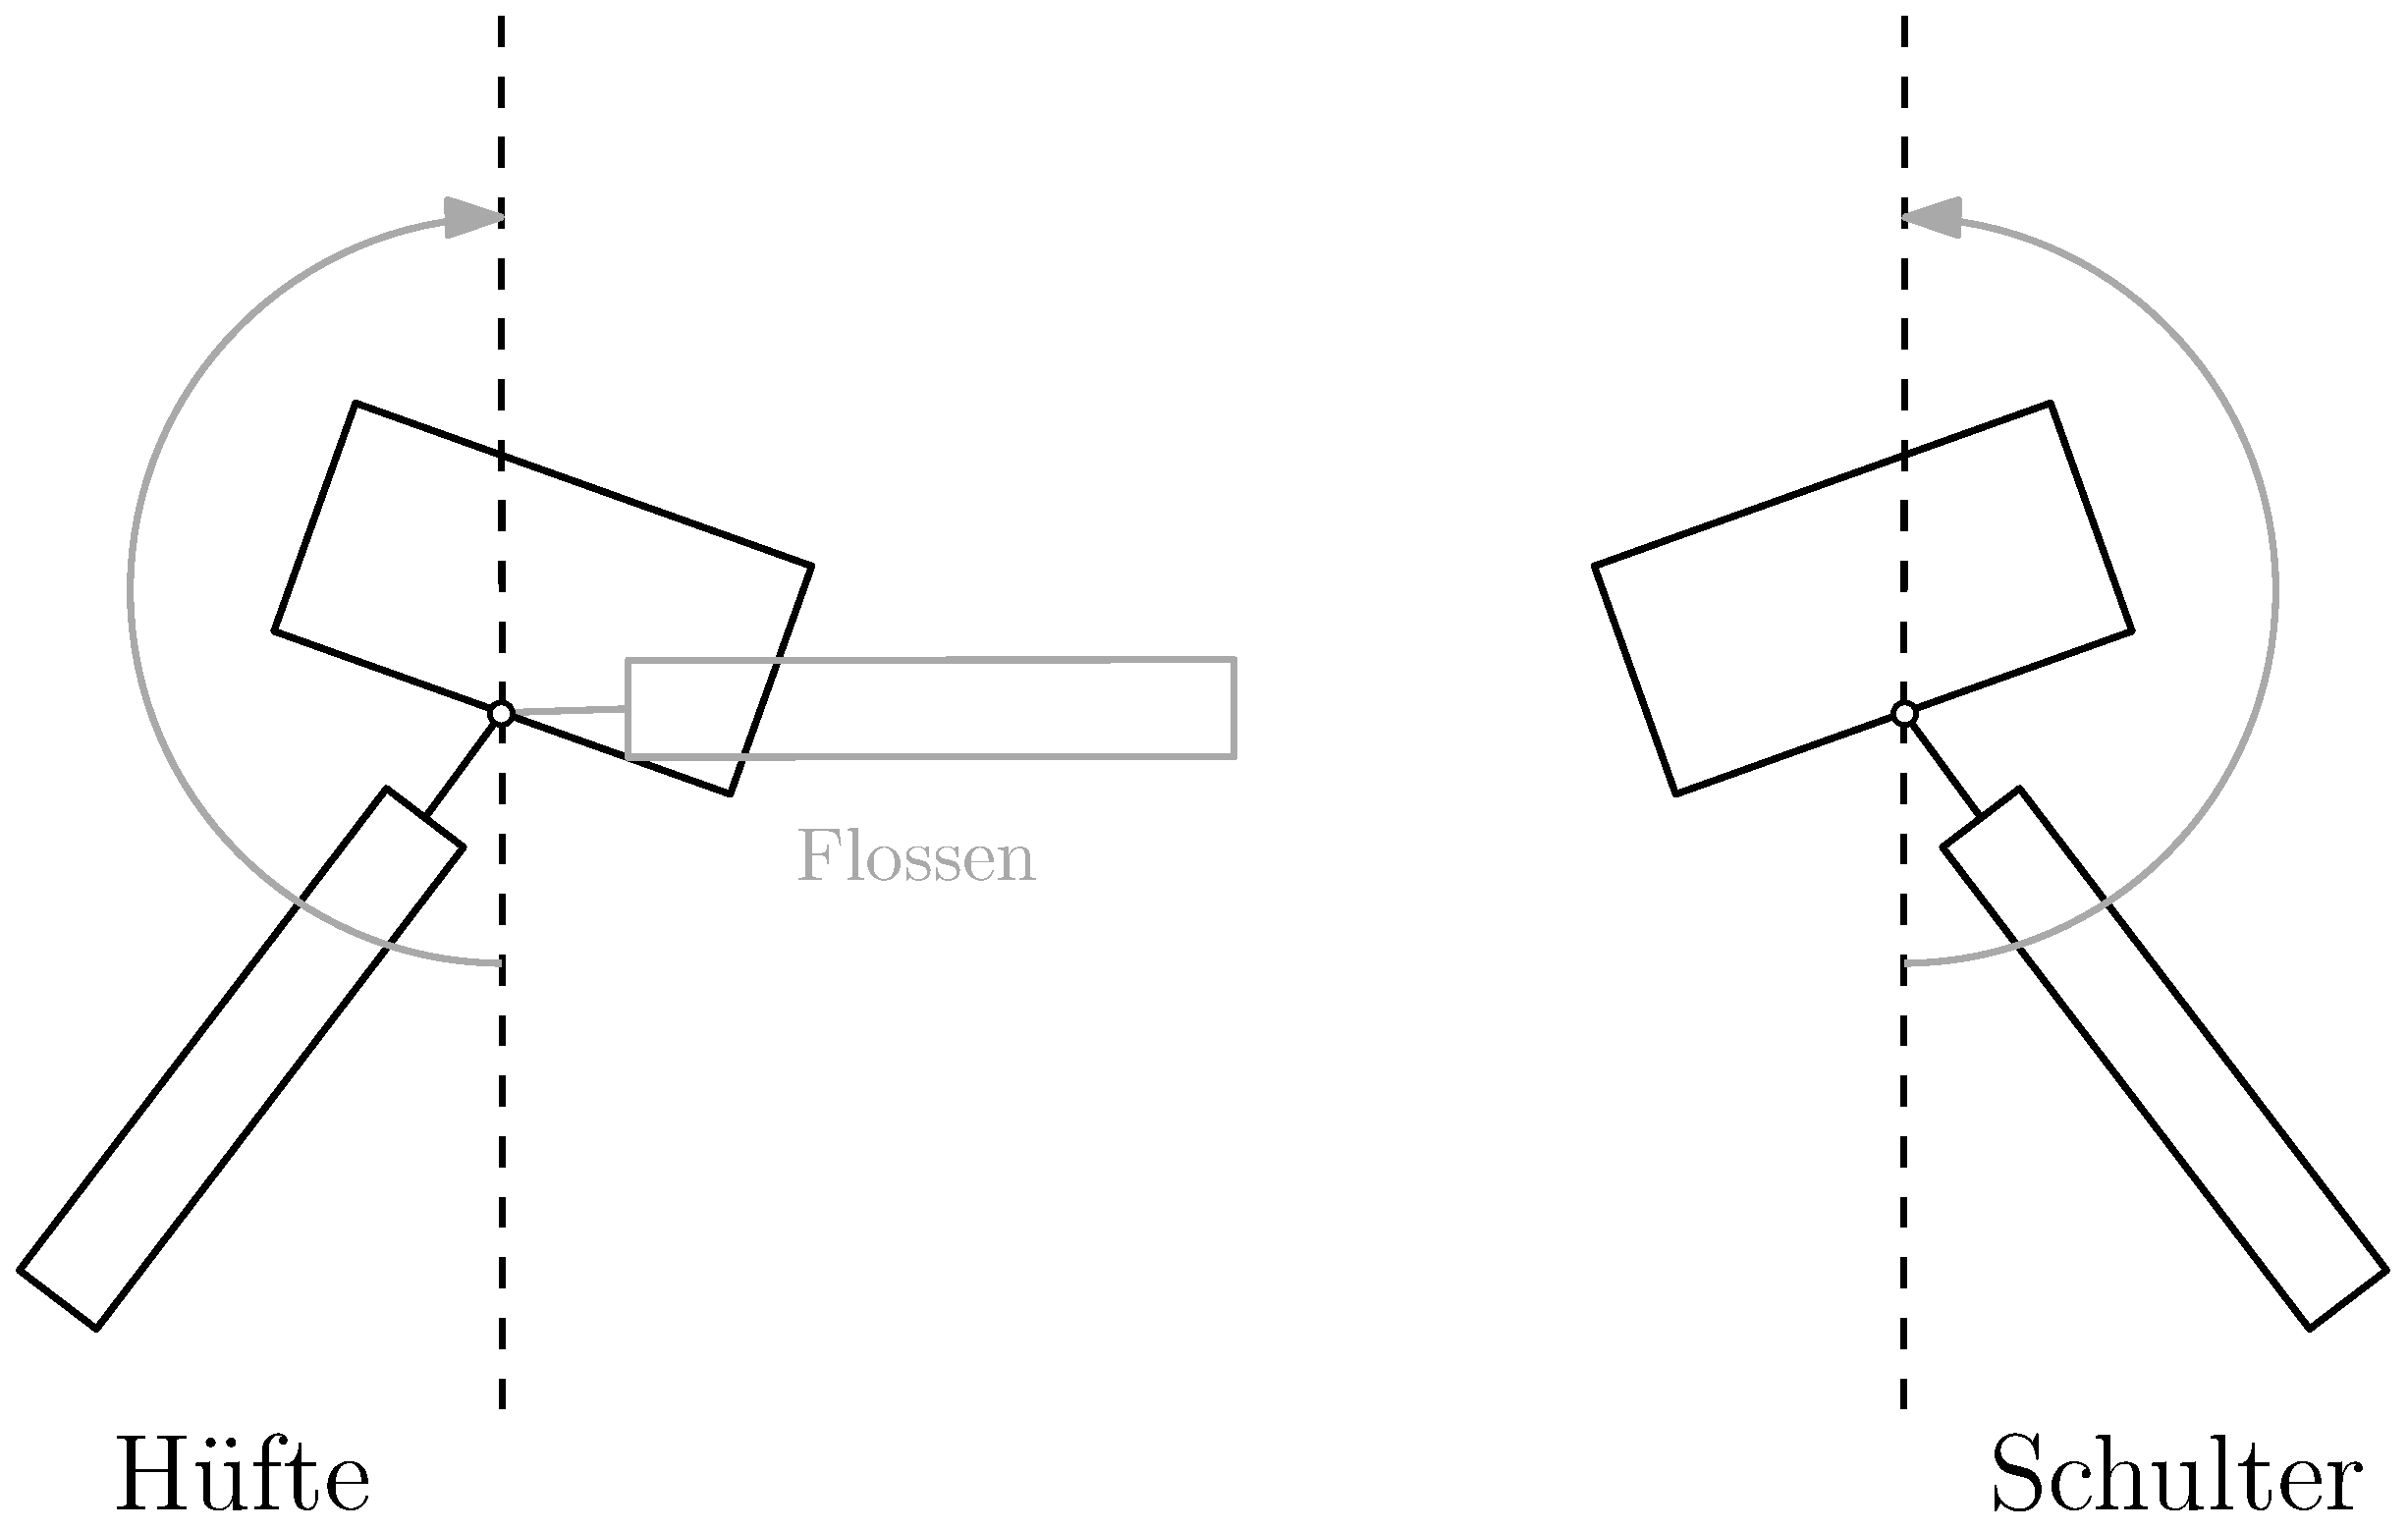
\includegraphics[width=0.5\textwidth]{graphics/twoDimJoints}}
  
  \caption{Visualisierung der Bewegungsradien für die Gelenke in Extremitäten. Darstellung in Seitenansicht (wie in Abbildung \ref{bauplan_skelett}). Es sind die möglichen Winkel für eine Ruheposition des Skeletts zu sehen. Unterarm, Unterschenkel und Fuß können jeweils maximal die Verlängerung des darüberliegenden Knochens bilden und minimal komplett an ihm anliegen. Oberarm und Oberschenkel können nicht über die Senkrechte hinaus gedreht werden (außer bei Flossen).}
  \label{joints}
 \end{figure}


%-----------------------------------------------------
\section{Von Groß und Klein}
\label{bigAndSmall}

Dieser Abschnitt widmet sich der Frage nach Unterschieden und Gemeinsamkeiten von großen und kleinen Wirbeltieren. Kann man Wirbeltiere und ihre Skelette einfach vergrößern und verkleinern? Oder sind sie besonders an ihre Größe angepasst? Unterscheidet sich das Skelett einer Maus wesentlich von dem eines Elefanten?

% Extrema
Zunächst ein kurzer Überblick über die Dimensionen, in denen man sich hier bewegt:\\
Das größte und schwerste Wirbeltier ist der Blauwal, er kann bis zu $120$ Tonnen wiegen (siehe \ref{appendix_pca_weight}). Das aktuell kleinste bekannte Wirbeltier, mit einer Länge von $7$ bis $8$mm, ist der Frosch \emph{Paedophryne amauensis} \cite{smallestVertebrate}. Größe und Gewicht von Wirbeltieren kann also erheblich variieren.

% Probleme bei Skalierung
Wenn ein Tier, oder eine ganze Stammeslinie, wächst, so ändert sich die Größe gleichmäßig. Dieses Wachstum ist aber begrenzt. Der Grund dafür ist, dass die Oberfläche nicht proportional mit dem Volumen mitwächst. Beispielsweise produziert ein Säugetier Wärme proportional zu seinem Volumen. Es kann aber nur Wärme proportional zu seiner Oberfläche abgeben. Dadurch haben große Säugetiere eher Probleme damit Wärme abzugeben und kleine damit warm zu bleiben. \\
Ein ähnliches Problem tritt bei Knochen auf. Die Last, die ein Knochen tragen kann, ist ungefähr proportional zu seiner Querschnittsfläche. Das Skelett muss aber die komplette Masse des Körpers tragen.

% Lösungen für Skalierungen
Aus diesem Grund ist die Oberfläche sehr großer Tiere oft überproportional vergrößert. Bei Knochenquerschnitten ist das jedoch nicht unbedingt der Fall. Das Problem an dicken Knochen ist, dass sie den Bewegungsradius, \zb der Extremitäten, stark einschränken. Deshalb passen viele Tiere stattdessen ihre Körperhaltung und Aktivität an, um Spitzenkräfte, wie Stöße oder Oszillationen, zu vermeiden.\\ (\cite{Vergleichende_Anatomie}, Kapitel 23)

Sehr große und sehr kleine Wirbeltiere können also nicht über einfaches Skalieren ineinander überführt werden. Dennoch ähneln sich ihre Skelette sehr.


%-------------------
\section{Mythologie}
\label{biology_mythology}

Dieser Abschnitt entfernt sich von tatsächlich vorkommenden Wirbeltieren und wirft einen Blick auf fantastische Tiere aus der Mythologie. Die Webseite \cite{vertebrateExtraLimbs} gibt einen guten Überblick über fiktive Wirbeltiere mit zusätzlichen Gliedmaßen. 

Bekannte Beispiele sind unter anderem:
\begin{itemize}
 \item \textbf{Zentauren} Sie haben einen Pferdekörper, aber statt eines Halses setzt ein menschlicher Oberkörper auf dem Schultergürtel auf. \cite{centaurs}
 
 \item \textbf{Pegasus} Der Pegasus hat ebenfalls den Körper eines Pferdes, aber auch Flügel, die zusätzlich zu den Vorderbeinen am Schultergürtel ansetzen. \cite{pegasus}
 
 \item \textbf{Asiatische Drachen} Sie haben einen langen schlangenartigen Körper mit oft mehr als vier Beinen.
\end{itemize}
